\documentclass[tikz,border=8pt,multi=tikzpicture]{standalone}
\usepackage{amsmath}
\usepackage{xcolor}
\usetikzlibrary{arrows.meta, calc}

\definecolor{mainblue}{HTML}{001158}
\definecolor{accent}{HTML}{8592bc}
\definecolor{lightaccent}{HTML}{e7e9f2}

\tikzset{
  force/.style={-{Stealth[length=3mm]}, line width=1.2pt, color=mainblue},
  dim/.style={-{Stealth[length=2mm]}, line width=0.7pt, color=accent},
  member/.style={line width=1.4pt, color=mainblue},
  cut/.style={accent, dashed, line width=1.1pt},
  every node/.append style={font=\sffamily}
}

\newcommand{\festlager}[1]{
  \begin{scope}[shift={#1}]
    \draw[line width=1pt] (0,0) -- (-0.3,-0.5) -- (0.3,-0.5) -- cycle;
    \draw[line width=1pt] (-0.42,-0.5) -- (0.42,-0.5);
    \foreach \x in {-0.42,-0.24,...,0.42} {\draw[line width=0.4pt] (\x,-0.5) -- (\x-0.13,-0.68);}
  \end{scope}
}
\newcommand{\loslager}[1]{
  \begin{scope}[shift={#1}]
    \draw[line width=1pt] (0,0) -- (-0.3,-0.5) -- (0.3,-0.5) -- cycle;
    \foreach \x in {-0.18,0,0.18} {\draw[fill=white, line width=0.7pt] (\x,-0.6) circle (0.1);}
    \draw[line width=1pt] (-0.42,-0.72) -- (0.42,-0.72);
    \foreach \x in {-0.42,-0.24,...,0.42} {\draw[line width=0.4pt] (\x,-0.72) -- (\x-0.13,-0.9);}
  \end{scope}
}
\newcommand{\joint}[1]{\fill[mainblue] #1 circle (2.5pt);}

% the shared Warren-truss geometry: A(0,0) B(2,2) C(4,0) D(6,2) E(8,0)
\newcommand{\warrentruss}{
  \draw[member] (0,0) -- (4,0) -- (8,0);
  \draw[member] (2,2) -- (6,2);
  \draw[member] (0,0) -- (2,2) -- (4,0) -- (6,2) -- (8,0);
  \joint{(0,0)} \joint{(2,2)} \joint{(4,0)} \joint{(6,2)} \joint{(8,0)}
  \node[below left] at (0,0) {$A$};
  \node[left] at ($(2,2)+(-0.12,0.08)$) {$B$};
  \node[below] at (4,-0.05) {$C$};
  \node[above] at (6,2.05) {$D$};
  \node[below right] at (8,0) {$E$};
}

\begin{document}

% ================= Concept: Ritterschnitt (method of sections) =================
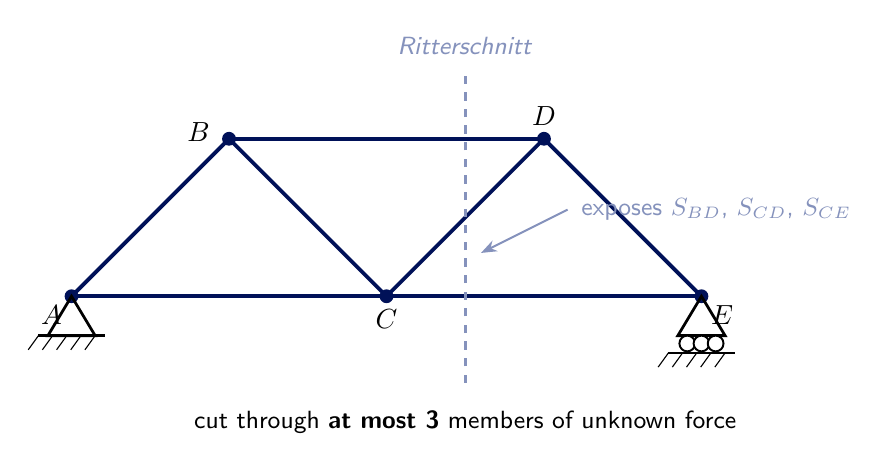
\begin{tikzpicture}
\warrentruss
\festlager{(0,0)}
\loslager{(8,0)}
\draw[cut] (5,-1.1) -- (5,2.9);
\node[accent, above] at (5,2.95) {\small \emph{Ritterschnitt}};
\node[align=center] at (5,-1.6) {\small cut through \textbf{at most 3} members of unknown force};
\draw[dim] (6.3,1.1) -- (5.2,0.55);
\node[accent, right] at (6.35,1.1) {\small exposes $S_{BD}$, $S_{CD}$, $S_{CE}$};
\end{tikzpicture}

% ================= Ex 6.1 problem: Warren truss, load at C =================
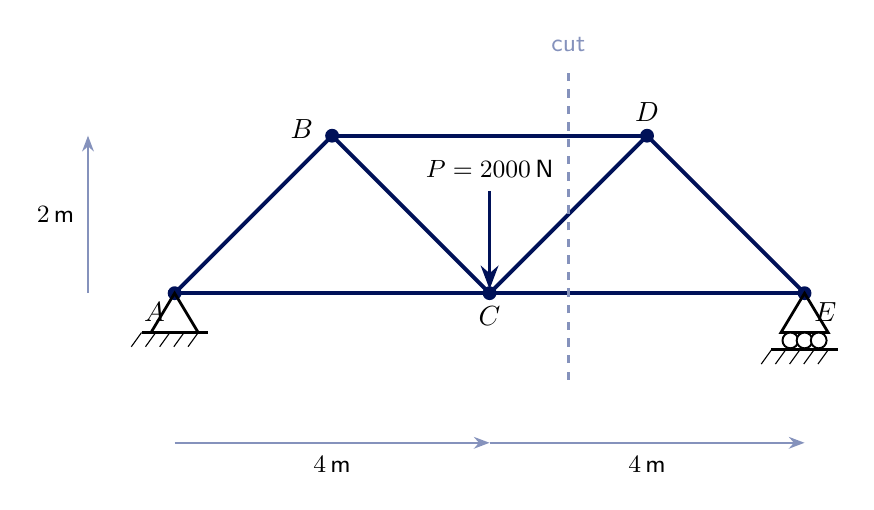
\begin{tikzpicture}
\warrentruss
\festlager{(0,0)}
\loslager{(8,0)}
\draw[cut] (5,-1.1) -- (5,2.9);
\node[accent, above] at (5,2.95) {\small cut};
\draw[force] (4,1.3) -- (4,0.05);
\node[above] at (4,1.35) {\small $P=2000\,\text{N}$};
\draw[dim] (0,-1.9) -- (4,-1.9);
\node[below] at (2,-1.95) {\small $4\,\text{m}$};
\draw[dim] (4,-1.9) -- (8,-1.9);
\node[below] at (6,-1.95) {\small $4\,\text{m}$};
\draw[dim] (-1.1,0) -- (-1.1,2);
\node[left] at (-1.15,1) {\small $2\,\text{m}$};
\end{tikzpicture}

% ================= Ex 6.1 FBD: right portion (D, E) =================
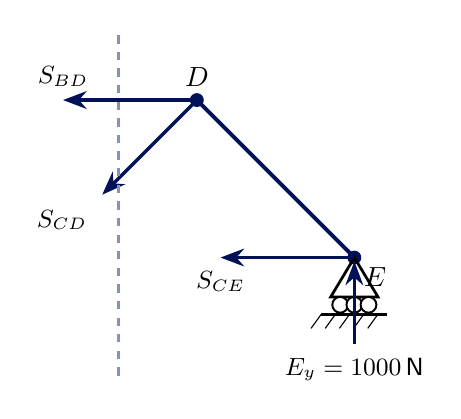
\begin{tikzpicture}
\draw[member] (6,2) -- (8,0);
\joint{(6,2)} \joint{(8,0)}
\loslager{(8,0)}
\node[above] at (6,2.05) {$D$};
\node[below right] at (8,0) {$E$};
\draw[force] (8,-1.1) -- (8,-0.05);
\node[below] at (8,-1.15) {\small $E_y=1000\,\text{N}$};
\draw[force] (6,2) -- ++(180:1.7);
\node[above] at (4.3,2.05) {\small $S_{BD}$};
\draw[force] (6,2) -- ++(225:1.7);
\node[below left] at ($(6,2)+(225:1.8)$) {\small $S_{CD}$};
\draw[force] (8,0) -- ++(180:1.7);
\node[below] at (6.3,-0.05) {\small $S_{CE}$};
\draw[cut] (5,-1.5) -- (5,2.9);
\end{tikzpicture}

% ================= Ex 6.2 problem: Warren truss, load at B =================
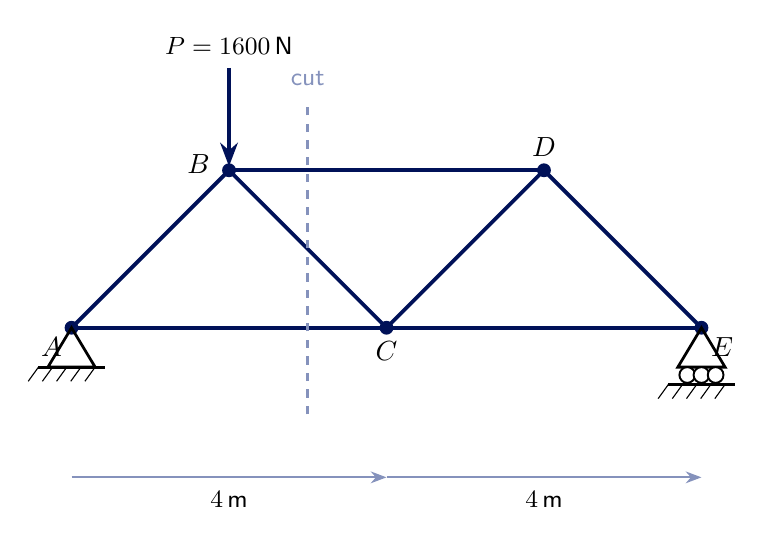
\begin{tikzpicture}
\warrentruss
\festlager{(0,0)}
\loslager{(8,0)}
\draw[cut] (3,-1.1) -- (3,2.9);
\node[accent, above] at (3,2.95) {\small cut};
\draw[force] (2,3.3) -- (2,2.05);
\node[above] at (2,3.35) {\small $P=1600\,\text{N}$};
\draw[dim] (0,-1.9) -- (4,-1.9);
\node[below] at (2,-1.95) {\small $4\,\text{m}$};
\draw[dim] (4,-1.9) -- (8,-1.9);
\node[below] at (6,-1.95) {\small $4\,\text{m}$};
\end{tikzpicture}

% ================= Ex 6.2 FBD: left portion (A, B) =================
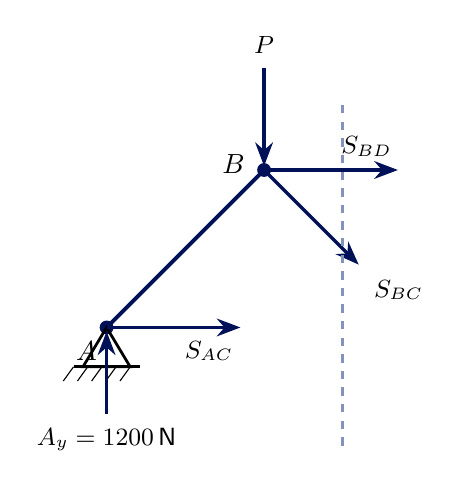
\begin{tikzpicture}
\draw[member] (0,0) -- (2,2);
\joint{(0,0)} \joint{(2,2)}
\festlager{(0,0)}
\node[below left] at (0,-0.05) {$A$};
\node[left] at ($(2,2)+(-0.12,0.08)$) {$B$};
\draw[force] (0,-1.1) -- (0,-0.05);
\node[below] at (0,-1.15) {\small $A_y=1200\,\text{N}$};
\draw[force] (2,2) -- ++(0:1.7);
\node[above] at (3.3,2.05) {\small $S_{BD}$};
\draw[force] (2,2) -- ++(-45:1.7);
\node[below right] at ($(2,2)+(-45:1.8)$) {\small $S_{BC}$};
\draw[force] (0,0) -- ++(0:1.7);
\node[below] at (1.3,-0.05) {\small $S_{AC}$};
\draw[force] (2,3.3) -- (2,2.05);
\node[above] at (2,3.35) {\small $P$};
\draw[cut] (3,-1.5) -- (3,2.9);
\end{tikzpicture}

\end{document}
